\input{standard.tex}

\ifpdf
  \DeclareGraphicsExtensions{.pdf, .jpg, .tif, .png}
  \pdfinfo{            
    /Title  (Architecture Notebook)
    /Author (PUM-grupp 1)
  }
\else
  \DeclareGraphicsExtensions{.eps, .jpg}
\fi

\title{Distribuerad wiki \\ Design}
\author{PUM-grupp 1}
\date{\today}

\begin{document}

\maketitle

\thispagestyle{empty}

\newpage

{\centering \Large{Dokumenthistorik\\}}

\vspace{10pt}
\begin{tabularx}{\textwidth}{ |l|l|X|l|l| }
  \hline
    \textbf{version} & \textbf{datum} & \textbf{utförda ändringar} & \textbf{utförda av} & \textbf{granskad} \\
	\hline 
  0.1 & 2009-02-12 &  Ett första utkast  & Alla & Alla   \\
	\hline	
  1.0 & 2009-03-09 & Alla klassdiagram ritade & Victor & Victor\\

  \hline
\end{tabularx}

\newpage

\setcounter{tocdepth}{2}
\tableofcontents
\newpage

\section{Design}

\section{Systemet}
Nedan följer designen för programvaran Dwiki.
\subsection{Språk och beroenden}
Dwiki är skrivet i python 2.6 och utnyttjar det distribuerade versionshanteringssystemet Bazaar. Som grafiskt bibliotek används wxPython.
\subsection{Överblick över systemet}
Programvaran består av följande delsystem som beskrivs mer i detalj senare i dokumentet.
\subsubsection{Interface}
\begin{itemize}
\item Model
\item Viewer
\end{itemize}
\subsubsection{klasser}
\begin{itemize}
\item Ett huvudfönster som är gränsnittet mot användaren.
\item En filhanterare som hanterar de filer och objekt systemet i huvudsak jobbar mot.
\item En objekttyp som är den datatypen filhanteraren och GUI:t jobbar emot.
\item Ett delsystem för att hantera den interna kommunikationen.
\item Ett delsysyem för att hantera den externa kommunikationen. 
\item Ett grupphanteringssystem som administrerar grupperna.
\item En krypterad socket som garanterar säker kommunikation.
\item Ett distruberat filhanteringssystem Bazaar.
\end{itemize}
Nedan följer en överskådlig bild på systemet.
 
\begin{figure}[ht]
  \centering
  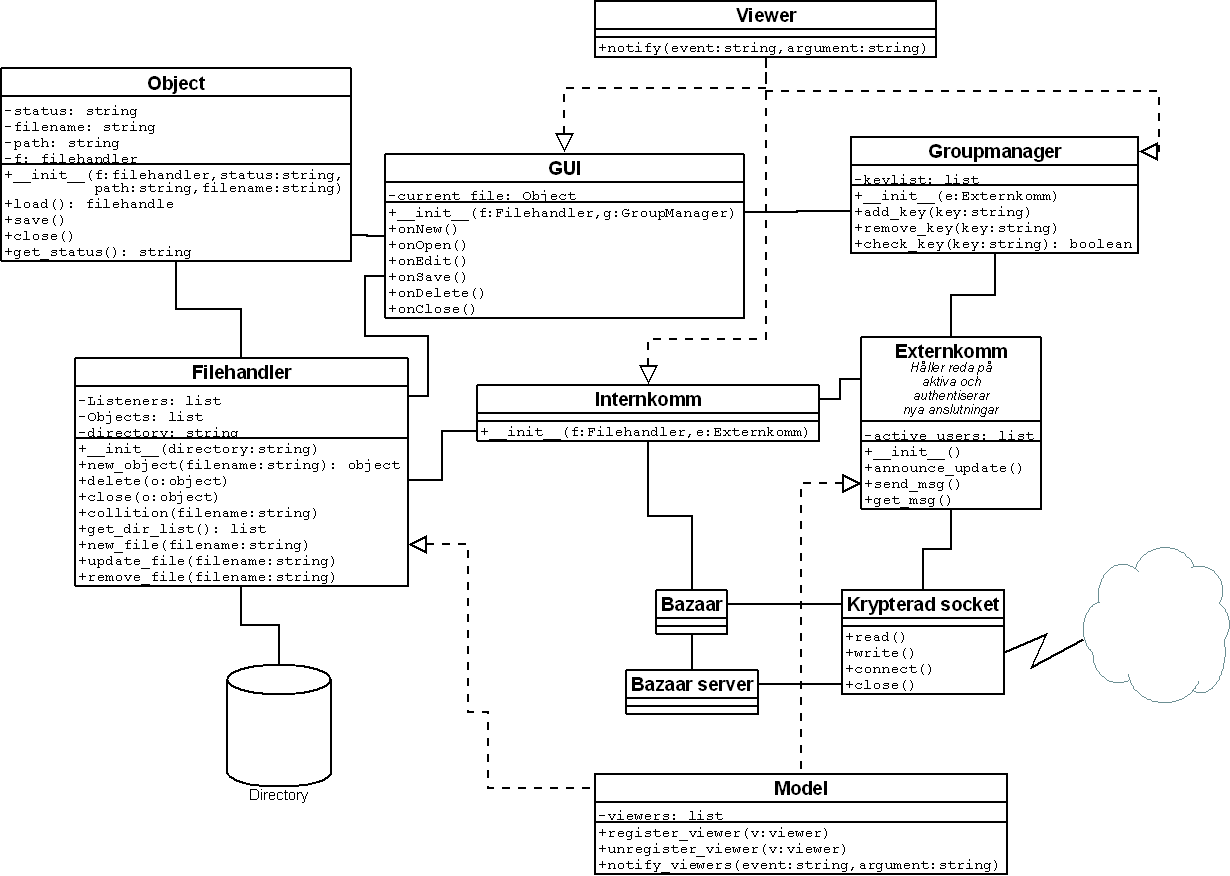
\includegraphics[width=160mm]{klassdiagram.png}
  \caption{Klassdiagram över systemet}
  \label{fig1}
\end{figure}
\clearpage
\subsection{Delsystem}
Nedan följer en mer detaljerad beskrivning över de olika delsystemen.

\subsubsection{Model}
Interfacet model är en del i MVC(Model View Controller) designmönstret. En model låter en viewer registrera sig så att den kan bli uppmärksammad på viktiga händelser av modellen. Detta är användbart då man vill minska beroenden mellan klasser.


\begin{tabular}{|l|p{10 cm}|}
\hline
\multicolumn{2}{|c|}{\textbf{Model}} \\
\hline
\multicolumn{2}{|c|}{viewers:list} \\
\hline
register\_viewer(v:viewer) & Metod för att registrera en viewer\\
unregister\_viewer(v:viewer) & Metod för att avregistrera en viewer\\
notify\_viewers(event:string, argument:string) & Metod för att uppmärksamma alla registrerade
viewers om en händelse\\
\hline
\end{tabular}

\subsubsection{Viewer}
Interfacet viewer är en del i MVC(Model View Controller) designmönstret. En viewer kan registrera sig hos en model och på så sätt bli uppmärksammad om viktiga händelser som modellen fått kännedom om.


\begin{tabular}{|l|p{10 cm}|}
\hline
\multicolumn{2}{|c|}{\textbf{Viewer}} \\
\hline
\hline
notify(event:string, argument:string) & Metod för att bli uppmärksammad om en händelse\\
\hline
\end{tabular}

\subsubsection{GUI}
GUI är systemets gränsnitt mot användaren. Den består av en texteditor och knappar för att interagera med resten av systemet.


\begin{tabular}{|l|p{10 cm}|}
\hline
\multicolumn{2}{|c|}{\textbf{GUI}} \\
\multicolumn{2}{|c|}{extends Viewer} \\
\hline
\multicolumn{2}{|c|}{current\_file:Filehandle} \\
\hline
\_\_init\_\_(f:filehandler,g:GroupManager) &konstruktor\\
OnNew(filename) & Metod för att skapa en ny artikel\\
OnOpen() & Metod för att ladda in och läsa en artikel \\ 
OnSave() & Metod för att spara en artikel \\
OnEdit() & Metod för att editera en artikel \\
OnClose() & Metod för att stänga en artikel \\
OnDelete() & Metod för att ta bort en artikel\\
notify(event:string) & Metod för att uppmärksamma en händelse\\
\hline
\end{tabular}

\subsubsection{Filehandler}
Filehandler är kopplinen mellan artikelfilerna och resten av systemet. Filhanteraren ser till så att nödvändiga parter blir informerade när en ändring eller en uppdatering på en fil har skett. 

\begin{tabular}{|l|p{10 cm}|}
\hline
\multicolumn{2}{|c|}{\textbf{Filehandler}} \\
\multicolumn{2}{|c|}{extends Model} \\
\hline
\multicolumn{2}{|c|}{Directory:string} \\
\multicolumn{2}{|c|}{Listeners:list} \\
\multicolumn{2}{|c|}{Objects:list} \\
\hline
\_\_init\_\_(directory) &konstruktor\\
new\_object(filename:string) : object & skapar och returnerar ett nytt object\\
new\_file(filename:string) & informerar filhanteraren om att det tillkommit en fil\\
update\_file(filename:string) & informerar filhanteraren om att en fil blivit uppdaterad\\
remove\_file(filename:string) & informerar filhanteraren om att en fil blivit borttagen\\
delete(o:object) & tar bort ett object\\
close(o:object) & stänger ett object\\
collition(filename:string) & informerar filhanteraren om en kollition\\
get\_dir\_list(): list & returnerar en lista med innehållet i katalogen\\
\hline
\end{tabular}

\subsubsection{Objekt}
Object är den klassen som kommer att representera alla aktiva artiklar. Ett objekt håller koll på statuset av artikeln och kan anropas med operationer på en artikel.

\begin{tabular}{|l|p{10 cm}|}
\hline
\multicolumn{2}{|c|}{\textbf{Object}} \\
\hline
\multicolumn{2}{|c|}{status: string} \\
\multicolumn{2}{|c|}{filename: string} \\
\multicolumn{2}{|c|}{path: string} \\
\multicolumn{2}{|c|}{f:filehandler} \\
\hline
\_\_init\_\_(f: filehandlerdirectory,status:string, &\\
path:string,filename:string) &Konstruktor, ställer in filehandler,status,path och filnamn\\
load(): filehandle & Returnerar handtaget till artikeln \\
save() & sparar ner information i filen \\
close() & stänger artikelfilen\\
get\_status(): string & Returnerar status för objektet \\
\hline
\end{tabular}

\subsubsection{Interna kommunikationen}
InternKomm är gränsnittet mellan filhanteraren, Bazaar och den externa kommunikationen. InternKomm låter filhanteraren veta om någon fil blivit uppdaterad av Bazaar. Likaså låter den Bazaar och den externa kommunikationen veta om någon fil uppdaterats av filhanteraren.

\begin{tabular}{|l|p{10 cm}|}
\hline
\multicolumn{2}{|c|}{\textbf{Internkomm}} \\
\multicolumn{2}{|c|}{extends Viewer} \\
\hline
\hline
\_\_init\_\_(f:Filehandler,e:Externkomm) &Konstruktor\\
\hline

\end{tabular}

\subsubsection{Externa kommunikationen}
Externkomm sköter den externa kommunikationen. Den skickar iväg meddelanden till andra användare om te.x uppdaterade filer eller nya användare i gruppen. Den hanterar också alla aktiva anslutningar.

\begin{tabular}{|l|p{10 cm}|}
\hline
\multicolumn{2}{|c|}{\textbf{Externkomm}} \\
\multicolumn{2}{|c|}{extends Model} \\
\hline
\multicolumn{2}{|c|}{active\_users:list} \\
\hline
\_\_init\_\_() &Konstruktor\\
announce\_update()& tillkännager användare om nya uppdateringar\\
send\_msg() & skickar ett meddelande till annan användare\\
recieve\_msg() & tar emot ett meddelande från annan användare\\
\hline

\end{tabular}

\subsubsection{Grupphantering}
Groupmanager hanterar den gruppen som wikin är medlem i. Den håller reda på vilka medlemmar som ingår i gruppen och låter administratörer lägga till eller ta bort användare ur gruppen genom att lägga till eller ta bort deras publika nycklar.

\begin{tabular}{|l|p{10 cm}|}
\hline
\multicolumn{2}{|c|}{\textbf{Groupmanager}} \\
\multicolumn{2}{|c|}{extends Viewer} \\
\hline
\multicolumn{2}{|c|}{keylist:list} \\
\hline
\_\_init\_\_(e:Externkomm) &Konstruktor\\
add\_key(key:string)& Lägger till en användares nyckel i gruppen\\
remove\_key(key:string)& Tar bort en användares nyckel ur gruppen\\
check\_key(key:string):boolean& kollar om en användares nyckel finns med i gruppen\\
\hline

\end{tabular}
\end{document}
